\subsection{Experimental Design} \label{sec:expDesign}
  Our evaluation is based on two benchmarks with significantly different access
  patterns. The first is quicksort (Qsort). This benchmark first allocates a
  large array of random numbers, and then sorts it using the well-known
  quicksort algorithm.  Quicksort is a divide and conquer algorithm that
  automatically partitions the input array into small local blocks before
  performing a final sort. This leads to excellent cache behavior and
  predictable access patterns.  Furthermore, by allocating the input array
  dynamically, quicksort performs no file I/O, so it is never blocked on I/O or
  other OS interactions.

  The other benchmark is a de-novo genome assembly benchmark (Gen). Gen begins
  by loading a large text file that represents raw genome data. Raw genome data
  consists of short, overlapping, sequences of base-pairs called "contigs", the
  goal is to align these overlapping contigs into a single contiguous sequence
  representing a genome. This is done by loading contigs into a large hash
  table and probing into it repeatedly to find matching sequences. This leads
  to very little locality and unpredictable access patterns. Furthermore, Gen
  performs file I/O on the input, which allows for more complex OS
  interactions.
\newline
\newline
  \begin{lstlisting}[frame=single]
# Data Schema
result = NamedTuple(
	'mean', # Mean results from 10 runs
	'std', # Standard deviation from 10 runs
)

# mean and std have the same set of keys
result.mean.keys
[ 't_run', 't_bookkeeping', 't_rmem_write',
  't_rmem_read', 'n_fault', 't_fault',
	'n_swapfault', 'n_pfa_fault', 'n_early_newq',
	'n_evicted', 'n_fetched', 'n_kpfad',
	't_kpfad', 'slowdown']

# Datasets
# Paging to remote memory in SW ('baseline')
base_res = ingest_run('raw/results_baseline.csv', 'rv')

# Paging using the PFA to real memblade
pfa_res = ingest_run('raw/results_pfa.csv', 'rv')

  \end{lstlisting}

\subsection{End-to-End Performance} \label{sec:fullPerf}
  The benchmarks were both run under a cgroup in Linux in order to reduce the
  available memory and emulate a system where applications would need to share
  limited local memory. This is the same mechanism that system administrators
  use today to control application memory consumption (e.g., in containers). In
  this experiment, we disable kpfad in order to isolate the batching of
  new-page management from the scheduling flexibility offered by kswapd's
  asynchrony.  The PFA was configured to allow up to 64 outstanding page faults
  before bookkeeping was performed.
  \newline
  \newline
  \lstinputlisting[frame=single]{real-pfa.patch}

  Both applications use 64MB of memory at their peak. We then
  varied the cgroup memory limit from 100\% (64MB) down to 25\% (16MB),
  triggering increasing levels of paging. For both benchmarks, the PFA reduces
  end to end run time by up to 1.4x.

  \begin{figure}[bht] \centering
    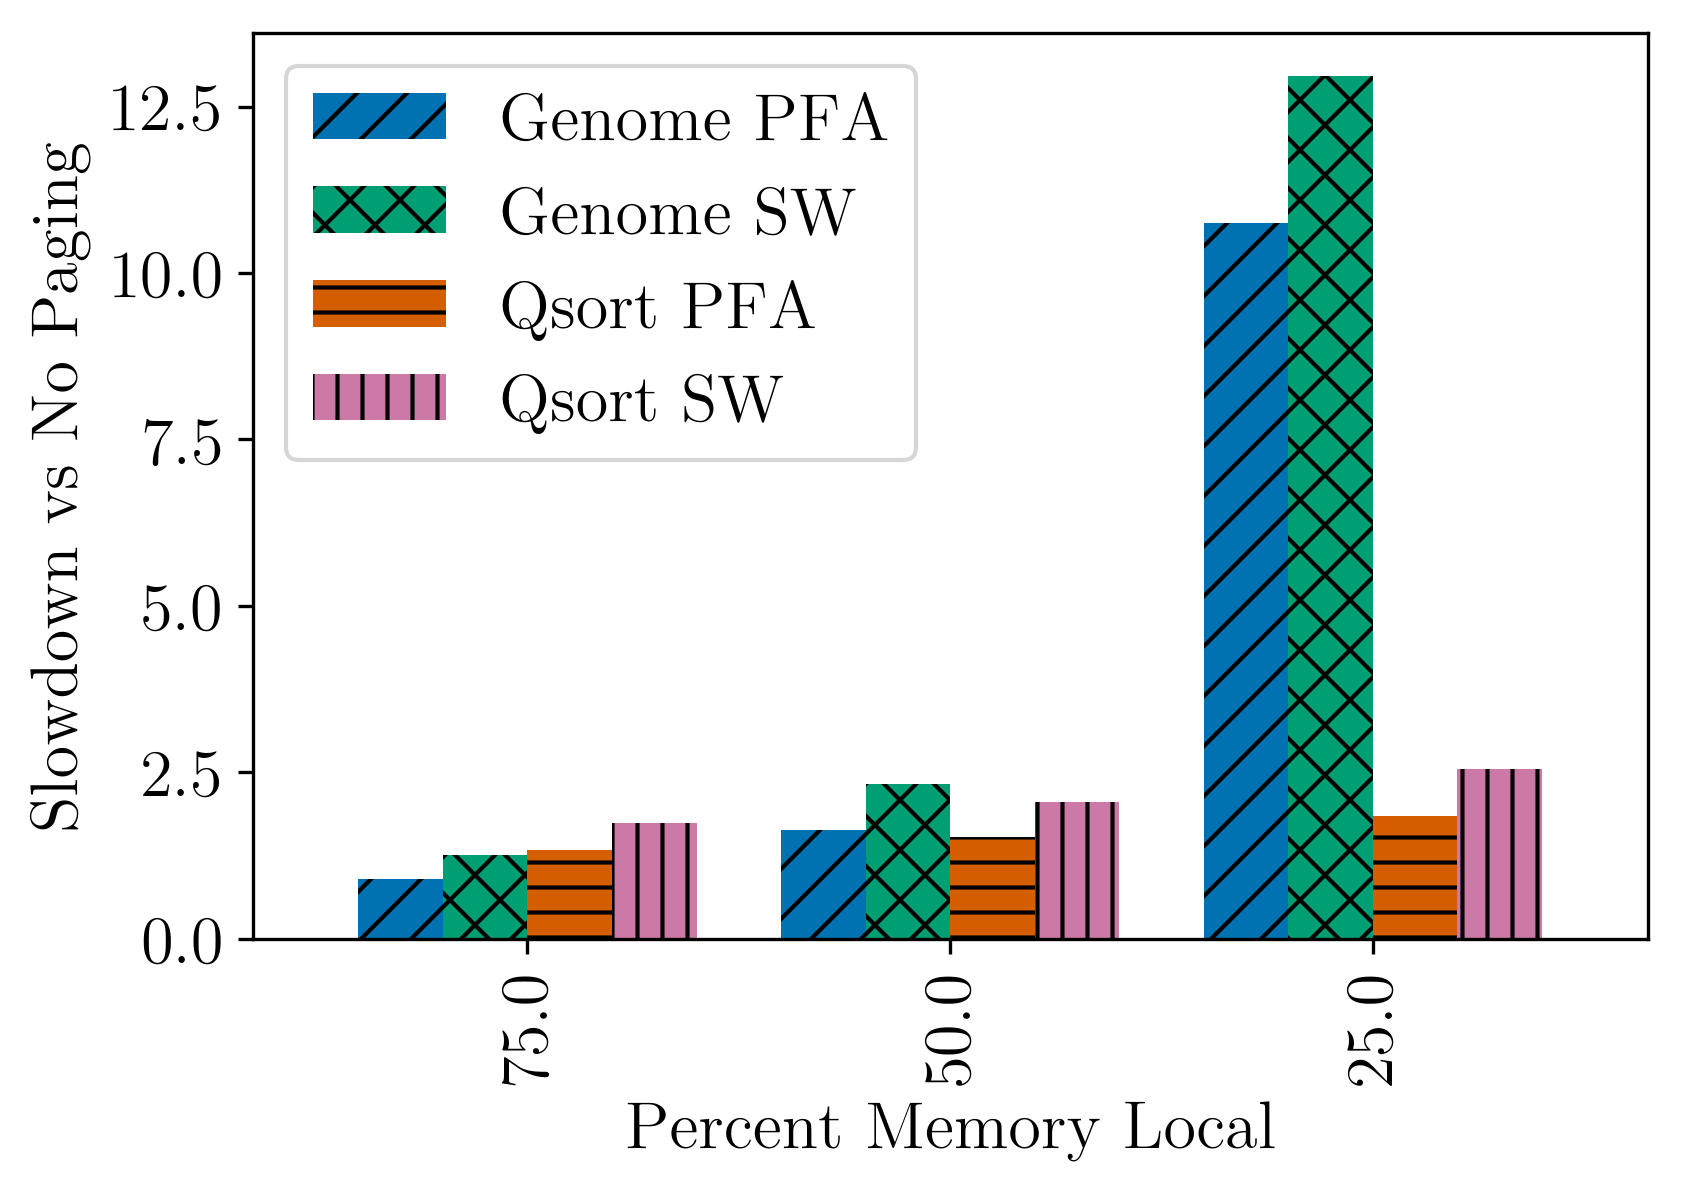
\includegraphics[width=0.5\columnwidth]{figs/perf_nokswapd.png}
    \vspace{+1cm}
    \caption{PFA vs Baseline without kswapd. Applications run approximately
    20-40\% faster when the PFA is enabled.}
    \label{fig:pfa_perf}
  \end{figure}

  \begin{figure}[bht] \centering
    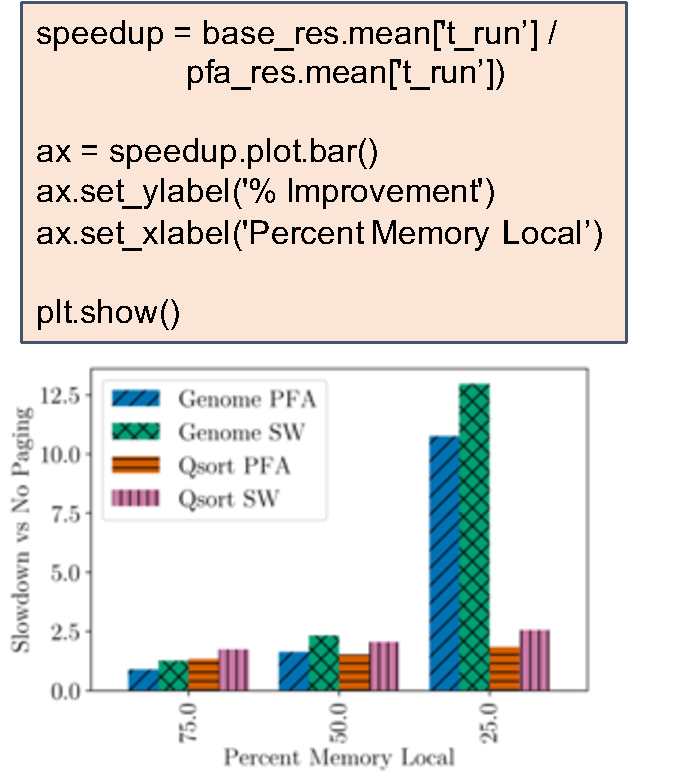
\includegraphics[width=0.5\columnwidth]{figs/perf_user.pdf}
    \vspace{+1cm}
    \caption{PFA vs Baseline without kswapd. Applications run approximately
    20-40\% faster when the PFA is enabled.}
    \label{fig:pfa_perf}
  \end{figure}

	\begin{figure}[bht] \centering
    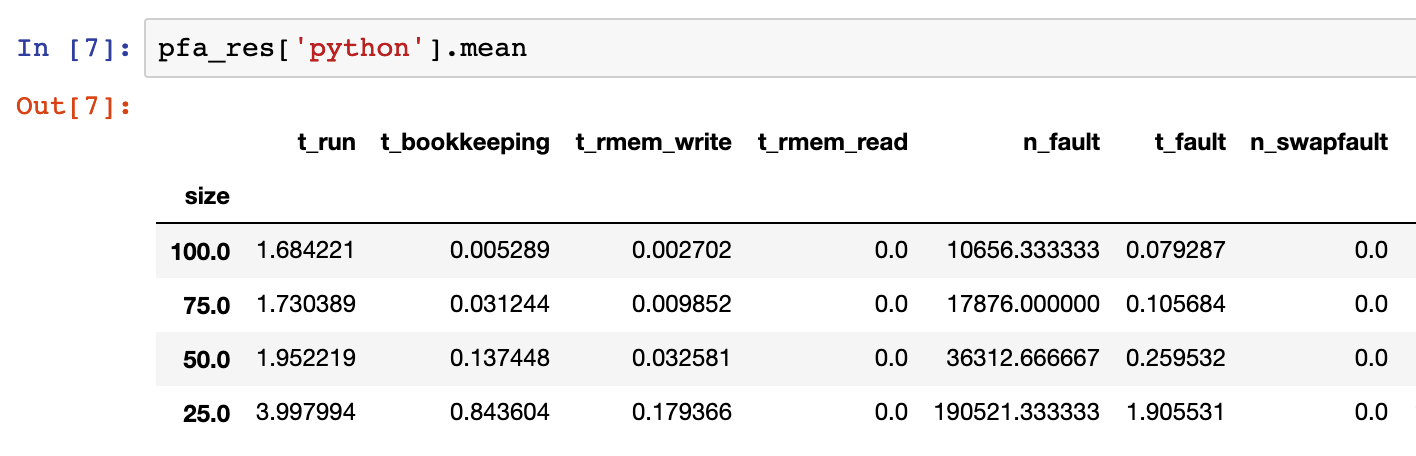
\includegraphics[width=0.8\columnwidth]{figs/perf_custom.png}
    \vspace{+1cm}
    \caption{PFA vs Baseline without kswapd. Applications run approximately
    20-40\% faster when the PFA is enabled.}
    \label{fig:pfa_perf}
  \end{figure}

% \subsubsection{Analysis}
%   We now analyze the sources of this performance improvement.
%   
%   \paragraph{Fetch Times}
%   We begin our analysis by looking at the key metric of average fetch time.
%   This is the time between when an application attempts to access a remote
%   page, and when it is able to continue processing. In this experiment, we use
%   a simplified memory blade and network implementation with a constant
%   \SI{4}{\micro\second} access latency in order to better understand local
%   overheads. Figure \ref{fig:fetch_breakdown} plots the time for accessing a
%   single remote page on an unloaded system. We classify time into four
%   categories:
%
%   \begin{outline}
%     \1 \textbf{Trap:} The time for the hardware to detect an invalid access and
%     context switch to the OS.
%     \1 \textbf{Proc:} The time spent processing the page locally (overhead).
%     \1 \textbf{NIC:} The time spent interacting with the network interface.
%     \1 \textbf{MemBlade:} The time spent on the network and in the memory
%     blade.
%   \end{outline}
%
%   Recall from Section \ref{sec:pfa} (and Figure \ref{fig:bookkeeping_timeline}
%   in particular) that the PFA moves some of this processing (especially
%   \textbf{Proc}) to an independent kernel thread; we account for this in a
%   later section. 
%
%   \begin{figure}[h] \centering
%     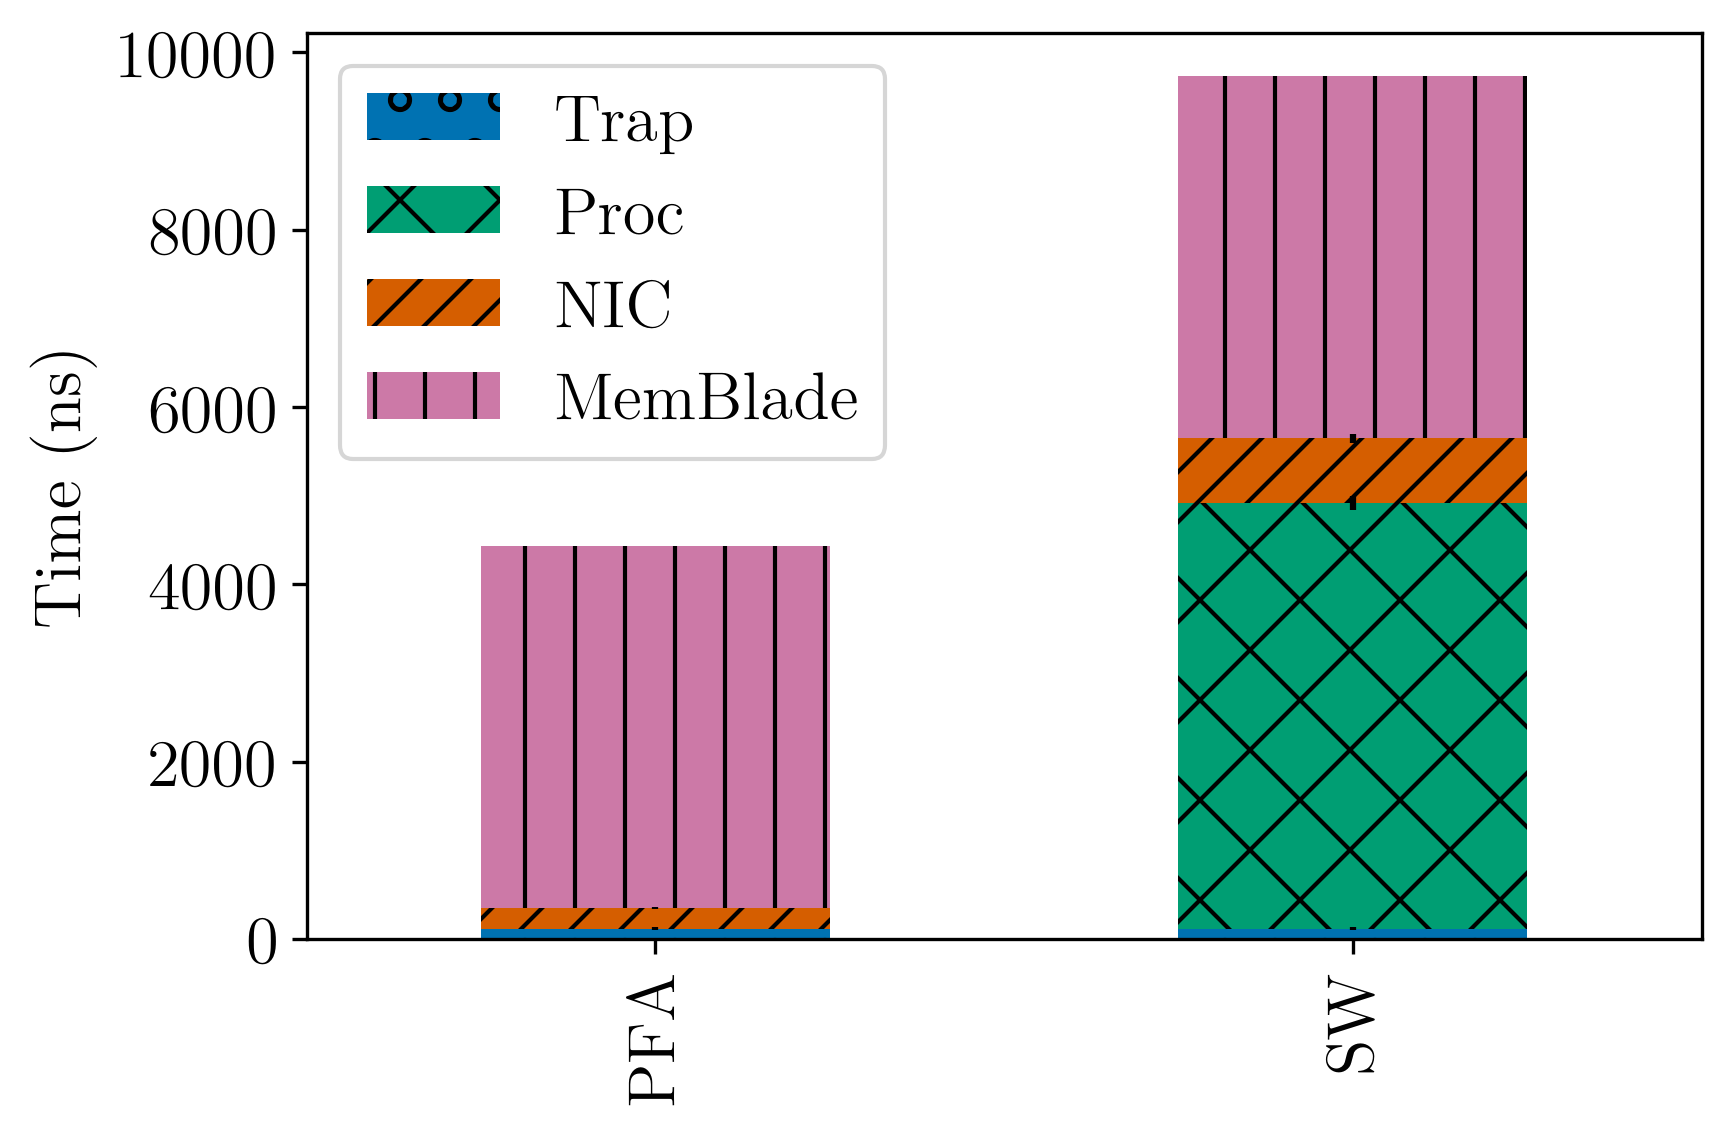
\includegraphics[width=0.8\columnwidth]{figs/fetch_breakdown.png}
%     \caption{Breakdown of time in fetching a single remote page. All data are 
%     the average of 10 runs. Error bars represent standard deviation (but are
%   almost too small to be seen). Note that local processing time (including
%   the trap and NIC interaction) only accounts for 8\% of time with the PFA, but
%   accounts for over 50\% of time for the baseline.}
%     \label{fig:fetch_breakdown}
%   \end{figure}
%
%   Note that the trap overhead is a very small fraction of total time (just
%   \SI{113}{\nano\second}). This is a result of using a simple in-order RISC
%   core like Rocket. It is likely that this overhead may be more significant on
%   a more complex architecture like server-grade x86 cores. Next, note that the
%   time spent on the network and in the memory blade accounts for less than half
%   the time in the baseline implementation, but completely dominates the PFA
%   fetch time. This effect will be even more pronounced as network and memory
%   blade performance improves. For example, if \textbf{MemBlade} time were
%   reduced to \SI{1129}{\nano\second} to simulate a \SI{1}{\tera\bit\per\second}
%   link with \SI{1}{\micro\second} round-trip latency (as predicted in Section
%   \ref{sec:firebox} for photonic networks), then client-side processing would
%   account for 83\% of time in SW but only 23\% of time with the PFA. Finally,
%   note that the \textbf{NIC} time in software is larger than the total time in
%   the PFA. We believe this is due to a more efficient hardware to hardware
%   interface between the PFA and the NIC. While not visible in the figure, the
%   actual PFA-specific processing takes only 1 cycle in hardware, the remaining
%   time is split between detecting and delivering the remote PTE to the PFA
%   (\textbf{Trap}), and interacting with the NIC (\textbf{NIC}). The total time
%   to fetch a page with the PFA is 2.2 times faster than in SW, but this does
%   not tell the whole story; The PFA does not eliminate the work that is done
%   during SW \textbf{Proc}, it simply moves it to another thread. Likewise, the
%   \SI{113}{\nano\second} trap overhead may seem small, but this does not
%   account for the effect that cache pollution from the handler has on the
%   application when it restarts.
%
%   \begin{figure}[h] \centering
%     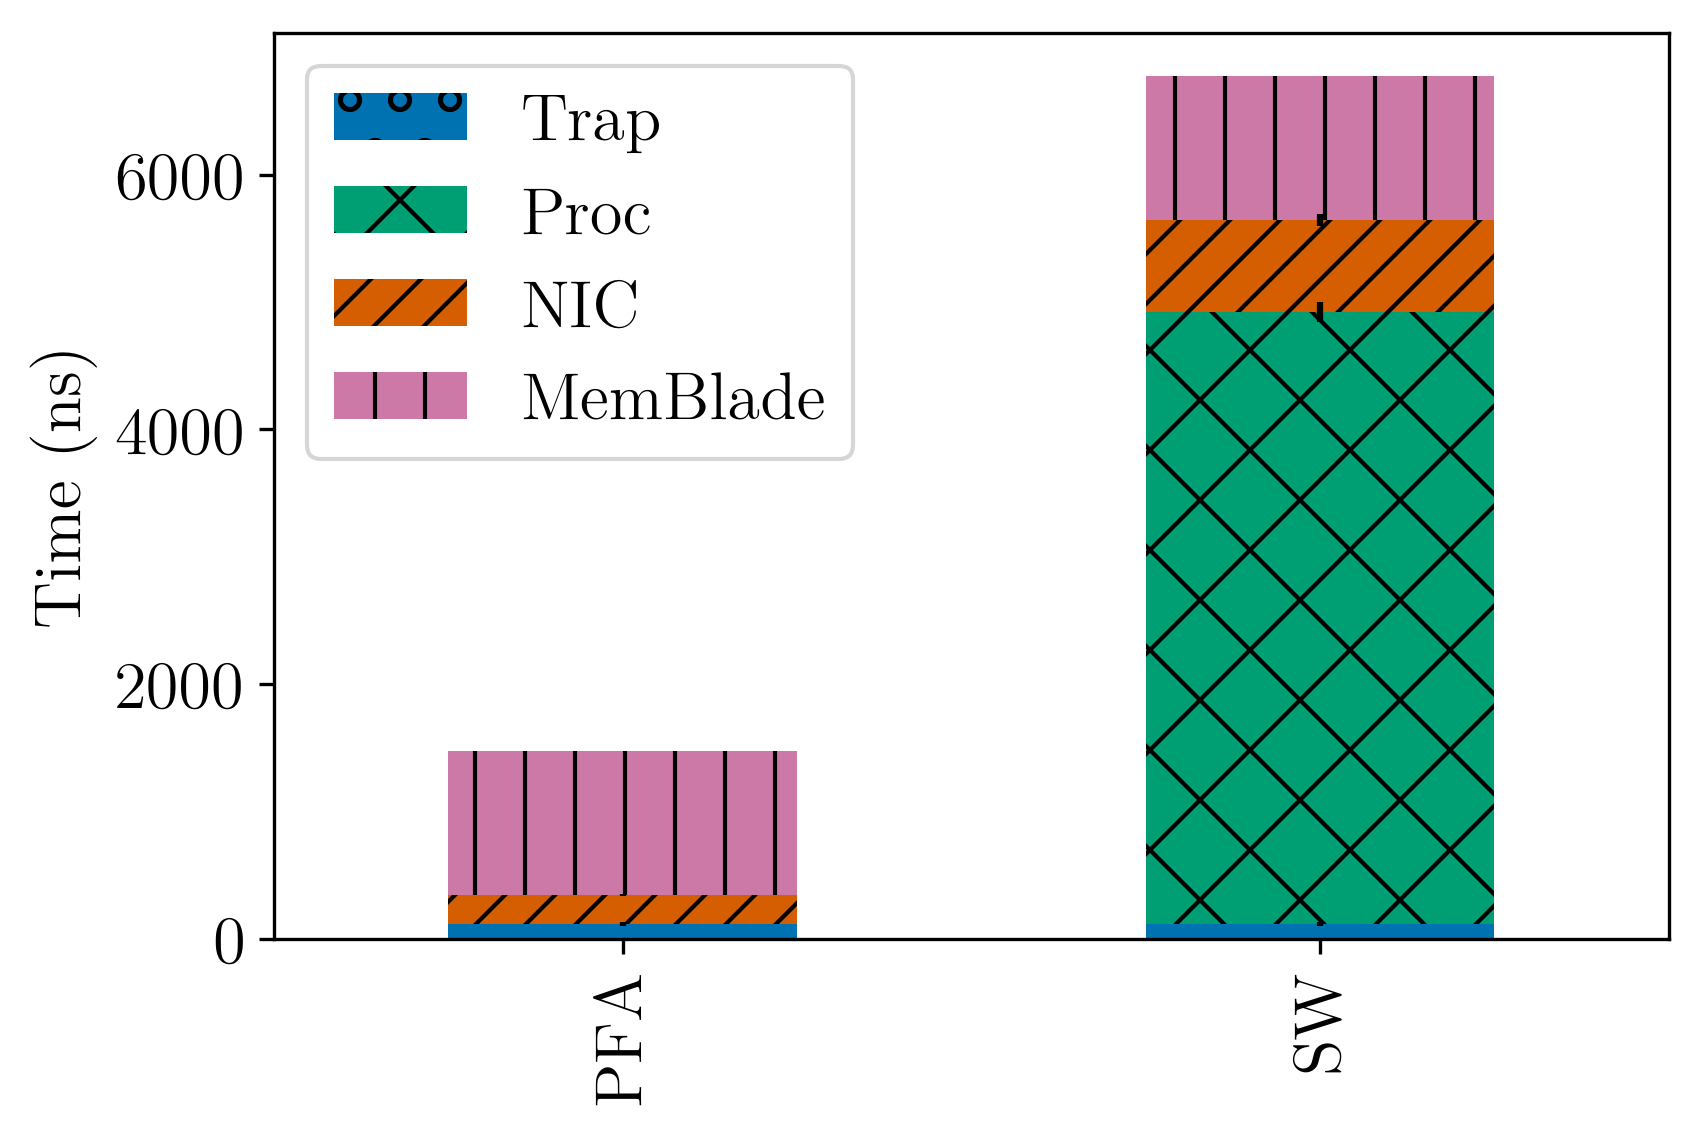
\includegraphics[width=0.8\columnwidth]{figs/fetch_breakdown_fastmem.png}
%     \caption{Breakdown of time in fetching a single remote page from a
%       hypothetical fast memory blade with \SI{1}{\micro\second} page read
%       latency. As network and memory technology improves, the relative benefit
%       of the PFA increases (from 2.2x faster with the baseline memory blade to
%       4.6x faster with the optimistic memory blade).}
%     \label{fig:fetch_breakdown}
%   \end{figure}
%
%   \paragraph{Total Page Faults}
%   One key function of the PFA is to reduce the number of page faults due to
%   paging. Recall from Section \ref{sec:pagingOverview} that there are many
%   causes for faults (e.g., to perform copy-on-write), in Figure
%   \ref{fig:pfa_swapfault} I plot the number of paging-related faults each
%   benchmark experiences as a fraction of total faults. The first thing to note
%   is that the number paging-related faults decreases by approximately 64 when
%   the PFA is used. This is because the PFA interrupts the OS to perform
%   bookkeeping only when its queues are full (every 64 fetches in this
%   experiment). However, these only account for 45\% of faults, even in the
%   worst-case (our simplest benchmark, Qsort) with 25\% local memory. The more
%   complex Gen benchmark has even fewer paging-related faults (as a fraction of
%   total). While there are certainly some savings due to fewer kernel crossings,
%   they are not frequent nor long enough to explain all the performance benefits
%   we see end-to-end.
%  
%   \begin{figure}[h] \centering
%     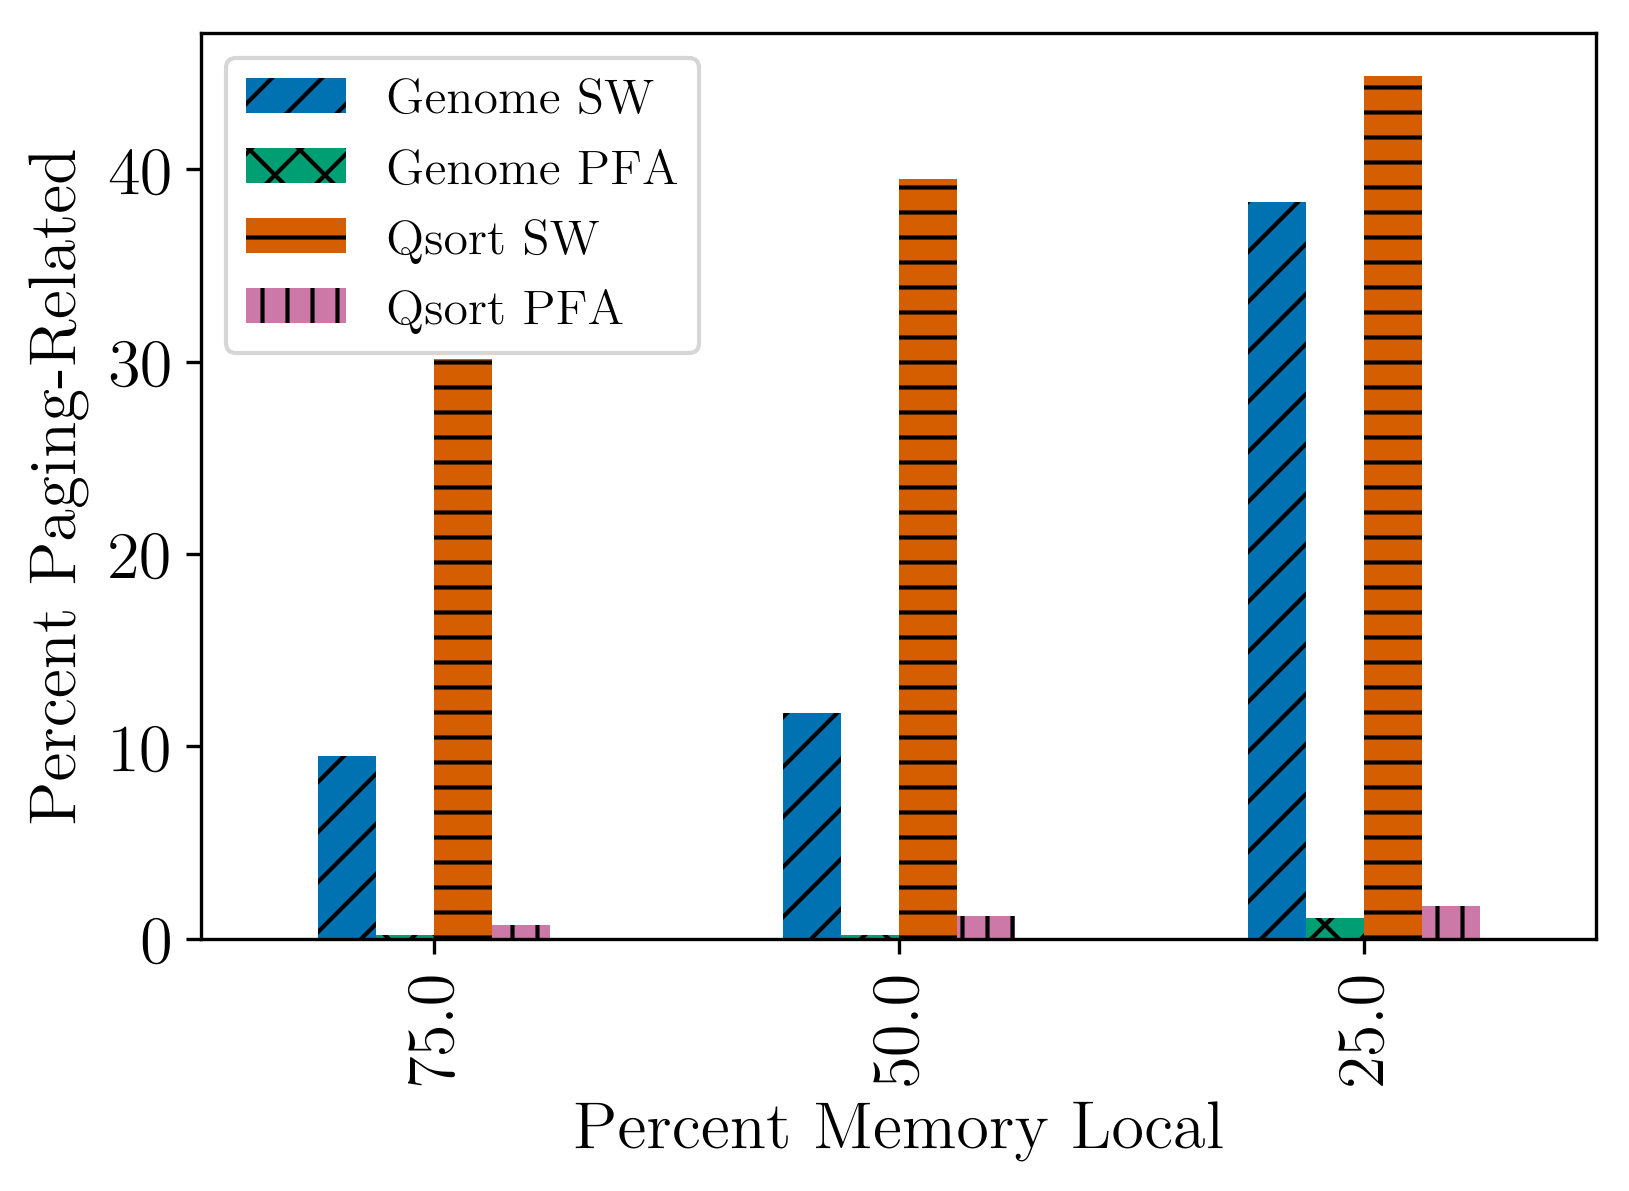
\includegraphics[width=0.9\columnwidth]{figs/swapfault.png}
%     \caption{Number of paging-related faults as a fraction of total faults
%     experienced.}
%     \label{fig:pfa_swapfault}
%   \end{figure}
%  
%   \paragraph{Bookkeeping Time}
%   While we do reduce the number of paging-related faults, the kernel still
%   needs to perform bookkeeping on the same number of pages. This batching
%   means that more work is performed per page fault with the PFA. Figure
%   \ref{fig:pfa_bk_prop} shows total time spent bookkeeping, regardless of the
%   number of page faults. What we see is that while the number of evicted pages
%   is the same in both configurations, using the PFA leads to a 2.5x reduction
%   in bookkeeping time on average. The same code path is executed for each
%   new page, but the PFA batches these events, leading to improved cache locality
%   for the OS, and fewer cache-polluting page-faults for the application. The
%   result is that, even in the worst case, the PFA spends less than half its
%   time handling paging-related faults, while the baseline spends about 80\%.
%
%   \begin{figure}[h] \centering
%     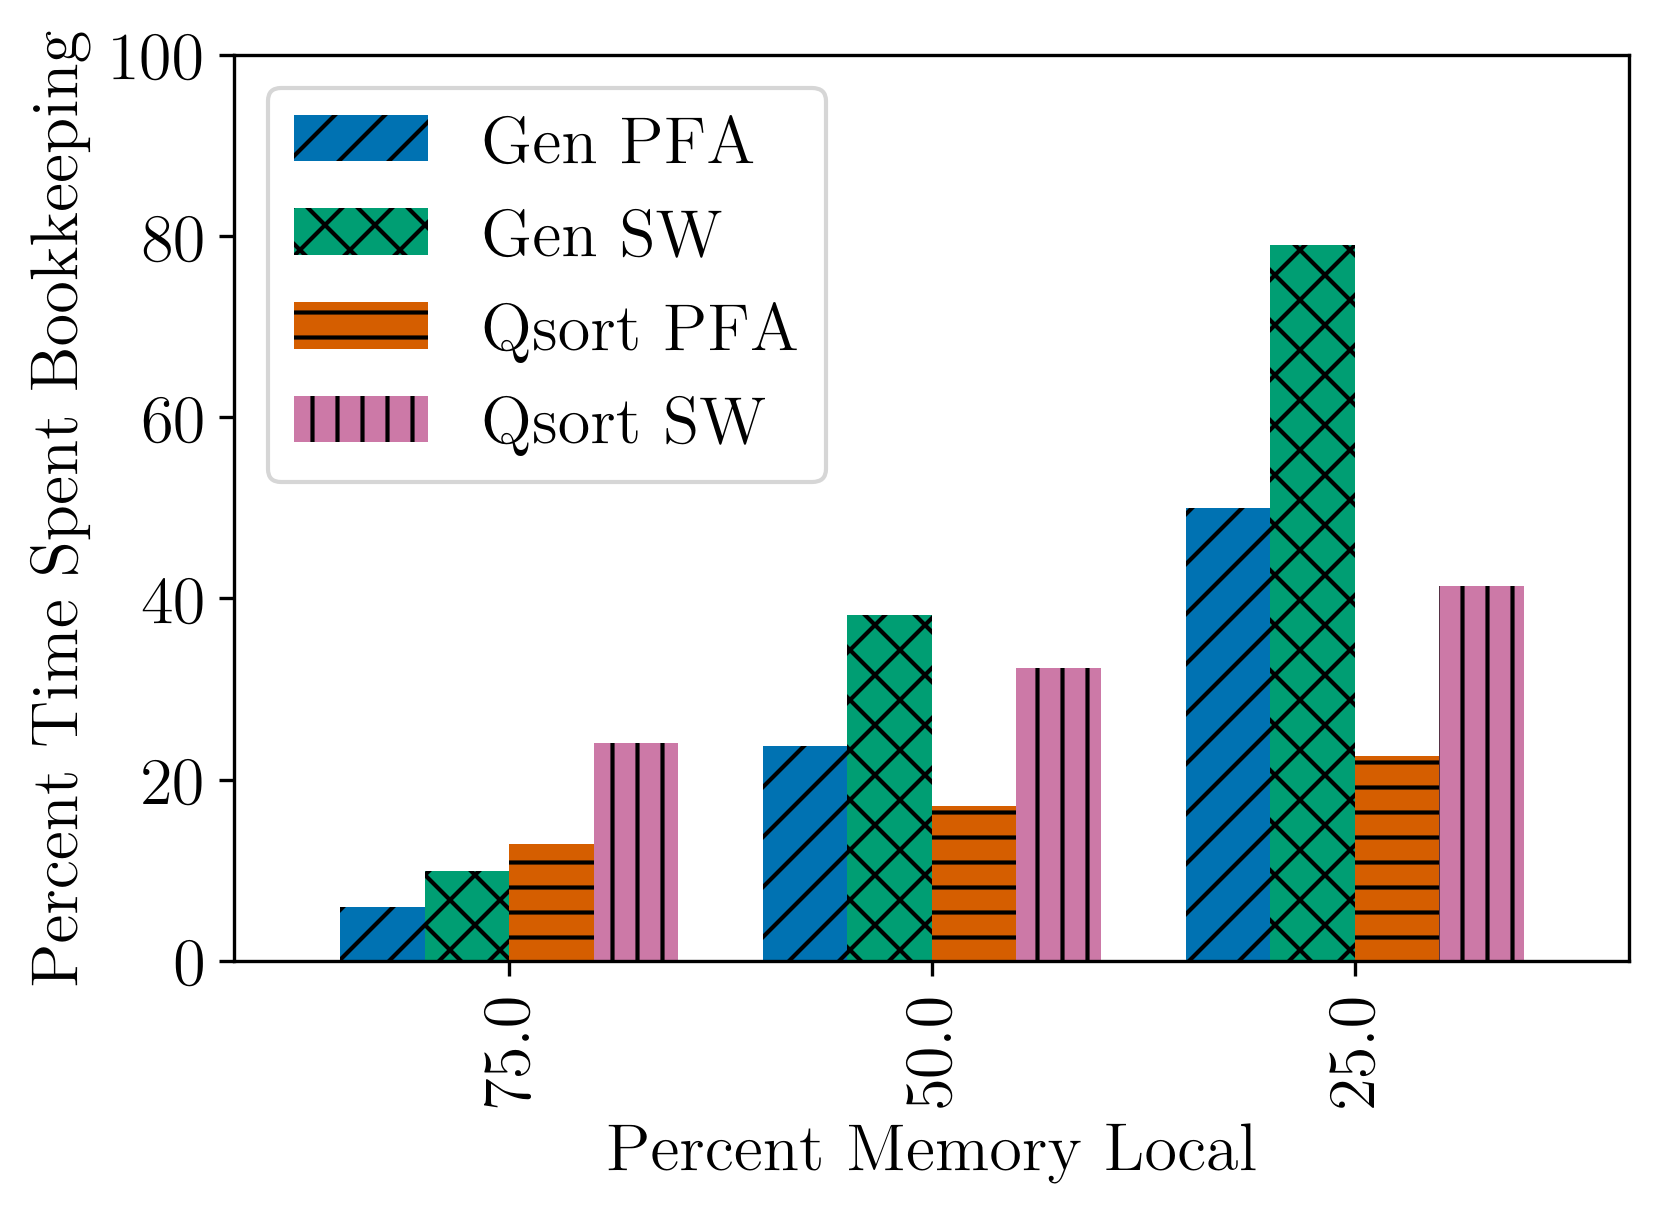
\includegraphics[width=0.8\columnwidth]{figs/bk_prop_all.png}
%     \caption{Proportion of Time Spent Bookkeeping}
%     \label{fig:pfa_bk_prop}
%   \end{figure}
%
%   \paragraph{Scaling}
%   Figure \ref{fig:pfa_total_speedup} shows the improvement in end-to-end
%   runtime due to the PFA on our applications. While the improvement is
%   significant (up to 40\%), the savings are constant (there is no asymptotic
%   improvement). This is because the PFA does not change any of the caching
%   algorithms, and therefor experiences the same number of faults. This means
%   that applications (such as Gen) that are not particularly cache-friendly can
%   see significant slowdowns in a disaggregated environment, even with the PFA.
%   Ultimately, the PFA pushes the boundaries of what is possible with cache-like
%   interfaces, but it cannot change their fundamental limitations. Applications
%   like Gen will need deeper changes to be viable on a disaggregated system.
%
%   \begin{figure}[h] \centering
%     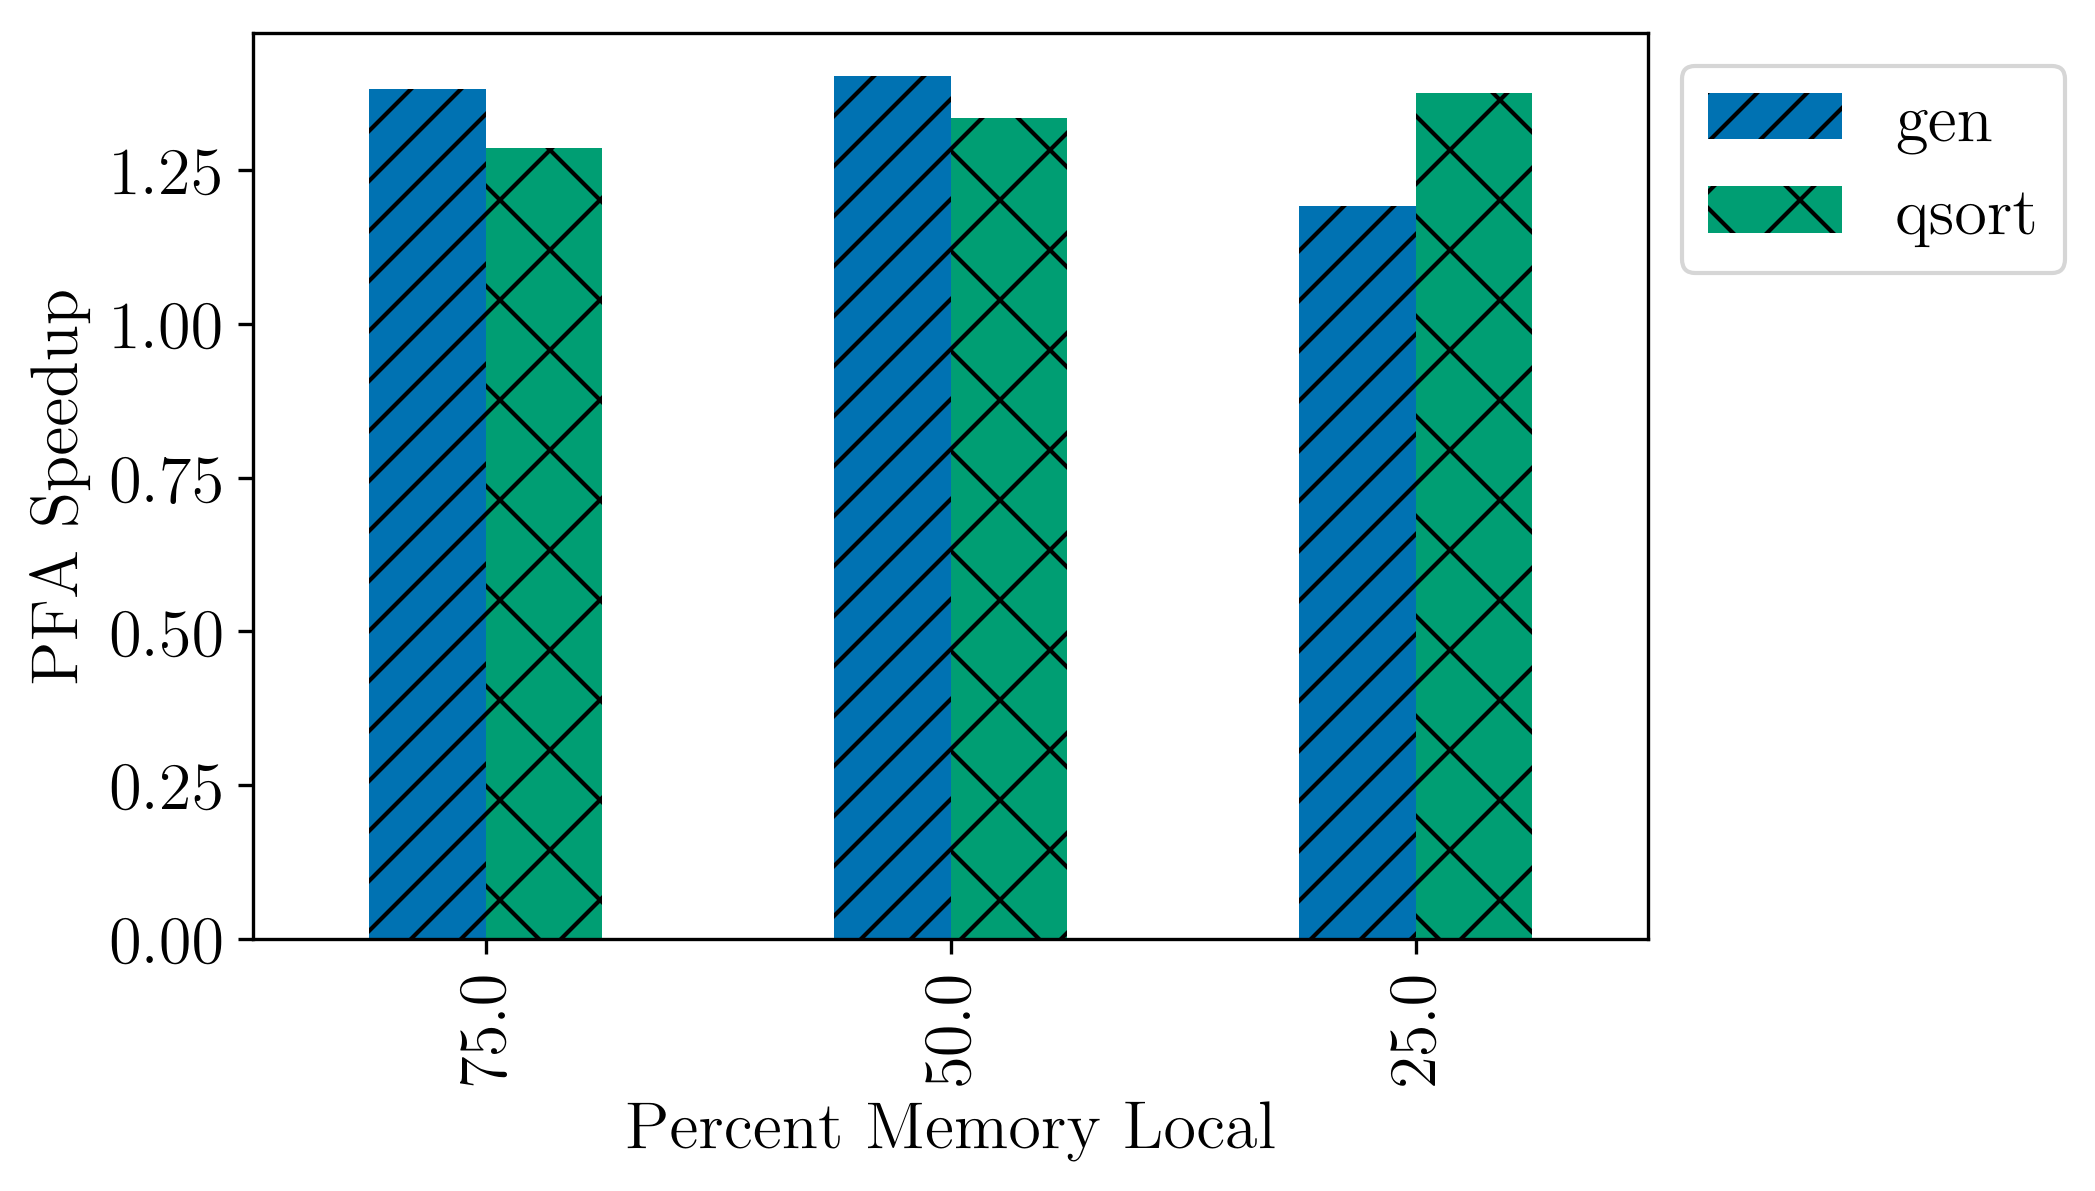
\includegraphics[width=0.8\columnwidth]{figs/total_speedup.png}
%     \caption{Total runtime improvement due to PFA}
%     \label{fig:pfa_total_speedup}
%   \end{figure}
%  
